
% This LaTeX was auto-generated from MATLAB code.
% To make changes, update the MATLAB code and republish this document.

\documentclass{article}
\usepackage{graphicx}
\usepackage{color}

\sloppy
\definecolor{lightgray}{gray}{0.5}
\setlength{\parindent}{0pt}

\begin{document}

    
    
\subsection*{Contents}

\begin{itemize}
\setlength{\itemsep}{-1ex}
   \item Part 1: DFT based spectral analysis
   \item Part 2: Periodogram-based spectral analysis
   \item Part 3: Spectrogram
\end{itemize}
\begin{verbatim}
% Alex Christenson EE125: Digital Signal Processing Matlab Project 5
% Performing spectral analysis on measured data from an ocean acoustics
% experiment
\end{verbatim}


\subsection*{Part 1: DFT based spectral analysis}

\begin{verbatim}
% Loading data from experiment
% Contains sample frequency (1.5 kHz) and xstart, which is the time series
% data for the start of the event, and xlater the time series data for
% after the event
load('Event59Data.mat')
x = xstart;

% Use FFT to perform spectral analysis for the signal
% Using a rectangular window
L = 512;
xRect = x(1:L).*rectwin(L);
XRect = fft(xRect,L);

% Using a hanning window
xHann = x(1:L).*hann(L);
XHann = fft(xHann,L);

% Plot the magnitude squared in dB of the two spectrums
f = Fs/2*linspace(0,1,L/2+1); % Create the frequency vector
XRectdB = mag2db(abs(XRect).^2); % Calculate mag squared and convert to dB
XHanndB = mag2db(abs(XHann).^2);

figure(1)

plot(f,XRectdB(1:L/2+1),f,XHanndB(1:L/2+1));

title('Spectrum of windowed signal, L = 512')
xlabel('Frequency (Hz)')
ylabel('Magnitude squared (dB)')
legend('Rectangular','Hanning')
axis([0 750 -240 -70])

% No, for the 512 window length you cannot clearly see that there are two
% tones around 200 Hz (at 198 and 201 Hz). For a window length of 512, the
% mainlobe width is (for rectangular window):
% 4pi/L = 4pi/512
% to convert from radians to Hz:
% 4pi/512 * Fs/2pi = 2*Fs/512 = 3000/512 = 5.8594 Hz.
% For the hanning window, mainlobe width is 8pi/M, which is twice that for
% the rectangular window, so the width is twice that for the
% rectangular window: 11.72 Hz.
% This tells us the bin width, and from this we can see that because the
% bin width is greater than the separation between the two frequencies,
% they will be unviewable.

% Repeating for L = 2048
L = 2048;
xRect2 = x(1:L).*rectwin(L);
XRect2 = fft(xRect2,L);

% Using a hanning window
xHann2 = x(1:L).*hann(L);
XHann2 = fft(xHann2,L);

% Plot the magnitude squared in dB of the two spectrums
f2 = Fs/2*linspace(0,1,L/2+1); % Create the frequency vector
XRectdB2 = mag2db(abs(XRect2).^2); % Calculate mag squared and convert to dB
XHanndB2 = mag2db(abs(XHann2).^2);

figure(2)

plot(f2,XRectdB2(1:L/2+1),f2,XHanndB2(1:L/2+1));

title('Spectrum of windowed signal, L = 2048')
xlabel('Frequency (Hz)')
ylabel('Magnitude squared (dB)')
legend('Rectangular','Hanning')
axis([0 750 -220 -40])

% Now that the window length is 2048 you can see the different toned
% frequencies. This makes sense because following the equation from the
% length equal to 512:
% 3000/2048 = 1.46 Hz, and for the Hann window, 2.93 Hz. This means the
% signals will be separable.

% Repeating for L = 2048
L = 8192;
xRect3 = x(1:L).*rectwin(L);
XRect3 = fft(xRect3,L);

% Using a hanning window
xHann3 = x(1:L).*hann(L);
XHann3 = fft(xHann3,L);

% Plot the magnitude squared in dB of the two spectrums
f3 = Fs/2*linspace(0,1,L/2+1); % Create the frequency vector
XRectdB3 = mag2db(abs(XRect3).^2); % Calculate mag squared and convert to dB
XHanndB3 = mag2db(abs(XHann3).^2);

figure(3)

plot(f3,XRectdB3(1:L/2+1),f3,XHanndB3(1:L/2+1));

title('Spectrum of windowed signal, L = 8192')
xlabel('Frequency (Hz)')
ylabel('Magnitude squared (dB)')
legend('Rectangular','Hanning')
axis([0 750 -200 -20])

% Looking at the graph from further increasing the number of points in the
% window, the SNR does look like it improves because you can see more
% significant spikes from where the tones we want to pick out are, so it
% looks like the SNR is improving.

% Using the normalization factors
% Also, I used a different normalization factor
normRect = sum(rectwin(L).^2);
normHann = sum(hann(L).^2);
XRectdB3 = mag2db(abs(XRect3).^2/normRect); % Calculate mag squared and convert to dB
XHanndB3 = mag2db(abs(XHann3).^2/normHann);

figure(4)

plot(f3,XRectdB3(1:L/2+1),f3,XHanndB3(1:L/2+1));

title('Normalized spectrum of windowed signal, L = 8192')
xlabel('Frequency (Hz)')
ylabel('Magnitude squared (dB)')
legend('Rectangular','Hanning')
% axis([0 750 -200 -20])

% Yay they match more closely now :)
\end{verbatim}

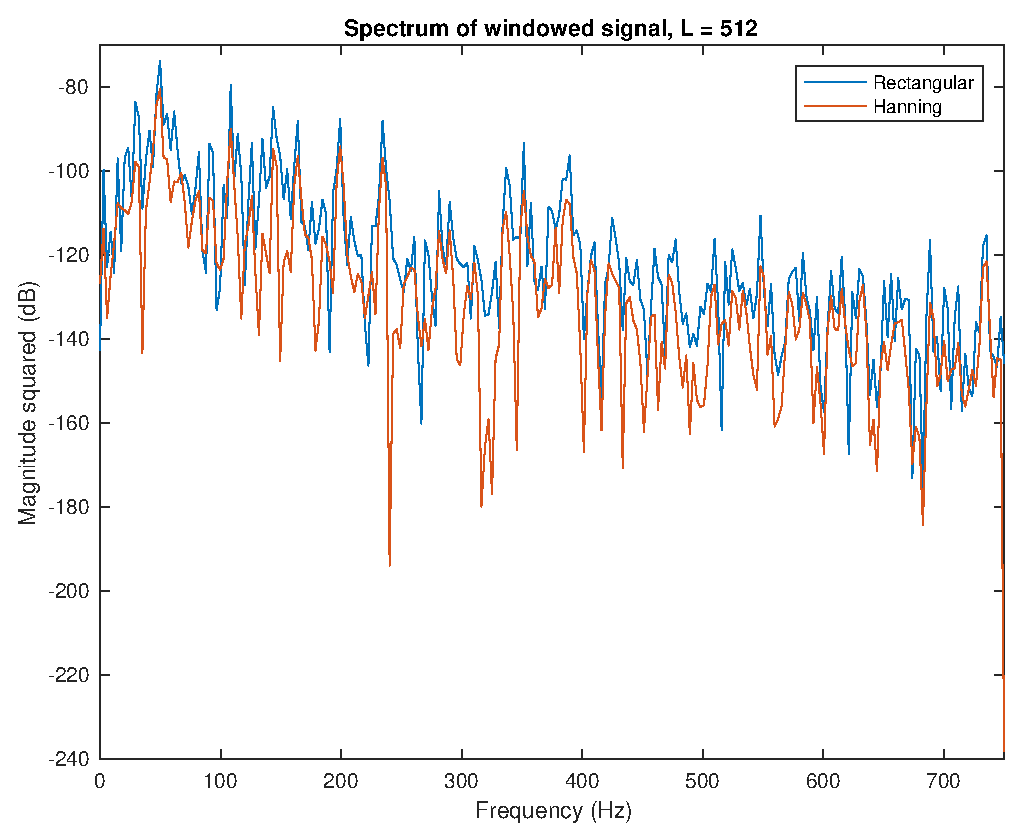
\includegraphics [width=4in]{EE125_Matlab5_01.eps}

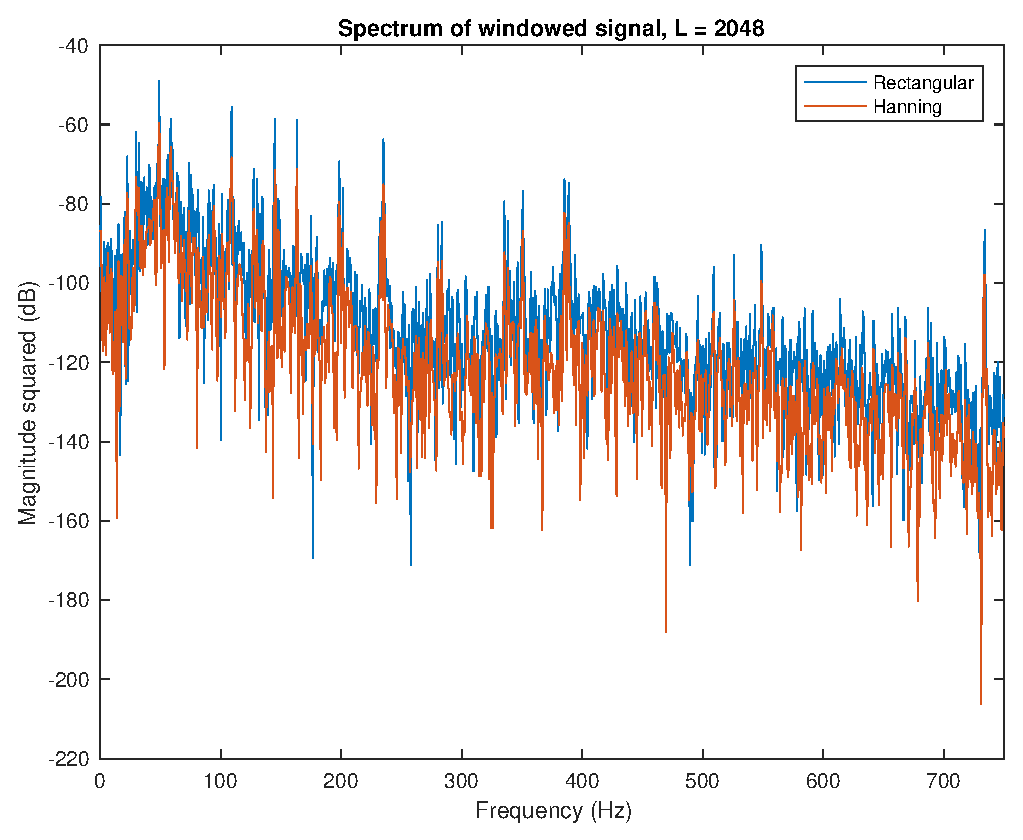
\includegraphics [width=4in]{EE125_Matlab5_02.eps}

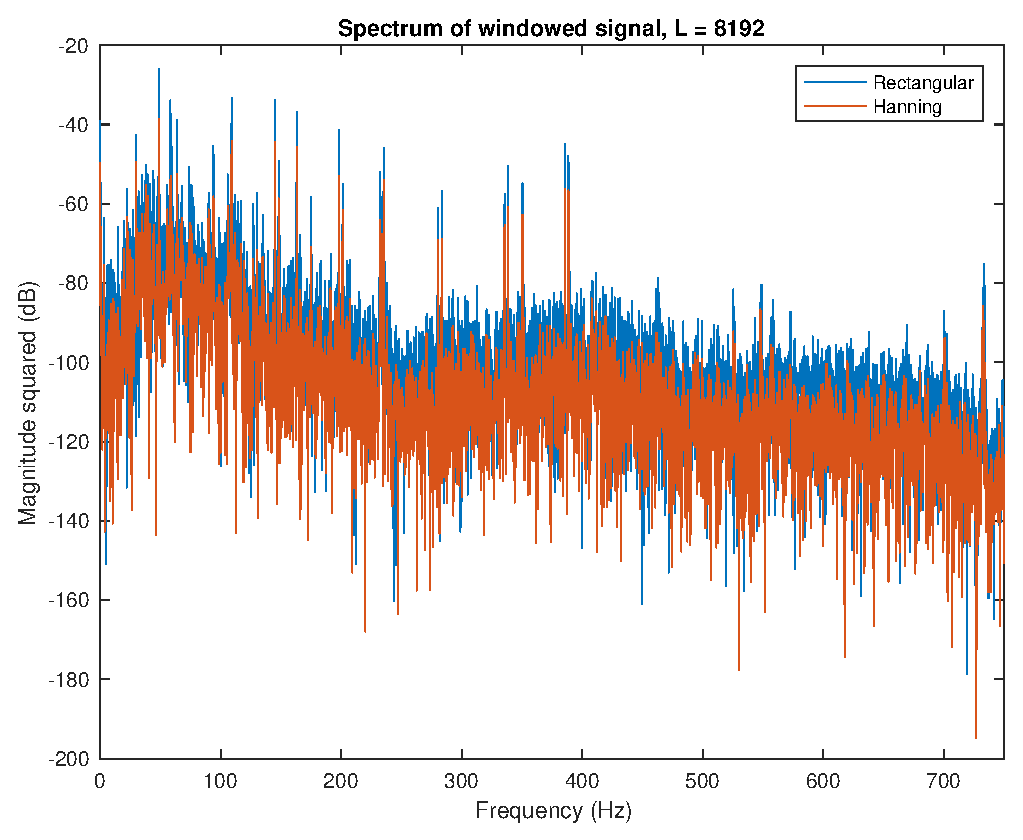
\includegraphics [width=4in]{EE125_Matlab5_03.eps}

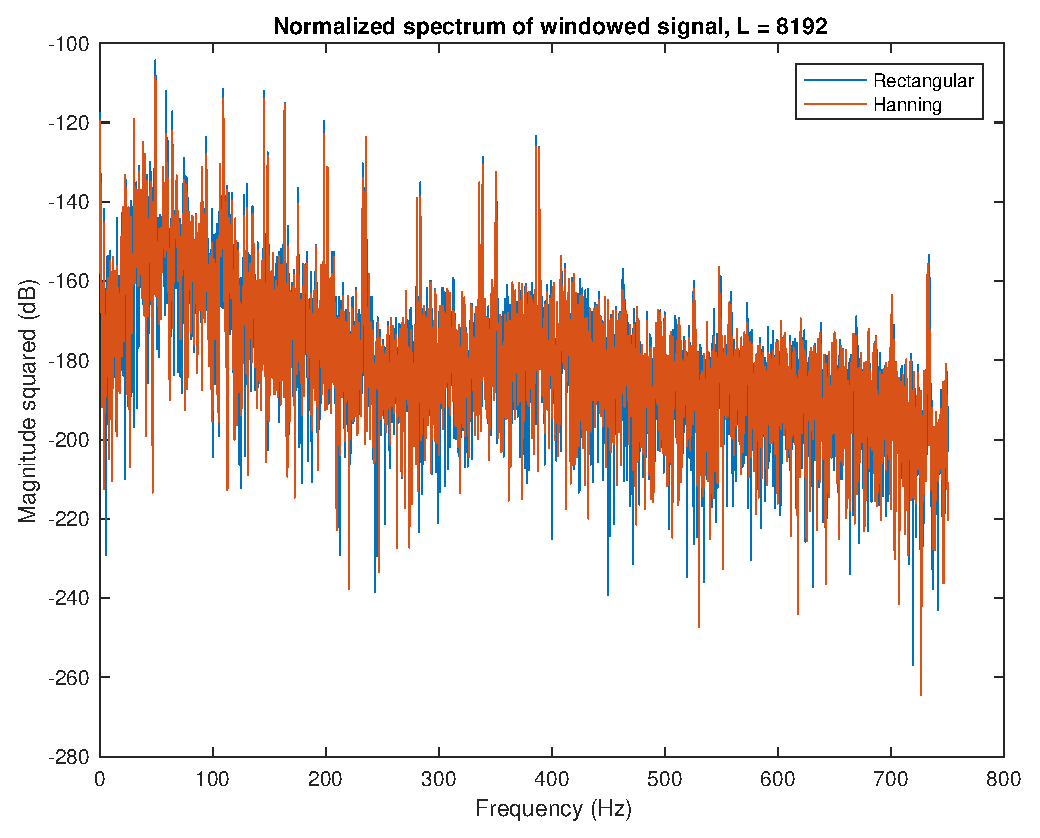
\includegraphics [width=4in]{EE125_Matlab5_04.eps}


\subsection*{Part 2: Periodogram-based spectral analysis}

\begin{verbatim}
L = 4096;
[bartRect,f1] = pwelch(x,rectwin(L),0,L,Fs);
[bartHann,f2] = pwelch(x,hann(L),0,L,Fs);

[rect50,f1] = pwelch(x,rectwin(L),0.5*L,L,Fs);
[hann50,f2] = pwelch(x,hann(L),0.5*L,L,Fs);

[rect75,f1] = pwelch(x,rectwin(L),0.75*L,L,Fs);
[hann75,f2] = pwelch(x,hann(L),0.75*L,L,Fs);

figure(5)
subplot(3,1,1)
plot(f1,mag2db(bartRect),f2,mag2db(bartHann));
title('Windowed signals of varying overlap, L=4096, 0% overlap')
xlabel('Frequency (Hz)')
ylabel('Power (dB)')
legend('Rectangular','Hanning')

subplot(3,1,2)
plot(f1,mag2db(rect50),f2,mag2db(hann50));
title('Windowed signals of varying overlap, L=4096, 50% overlap')
xlabel('Frequency (Hz)')
ylabel('Power (dB)')
legend('Rectangular','Hanning')

subplot(3,1,3)
plot(f1,mag2db(rect75),f2,mag2db(hann75));
title('Windowed signals of varying overlap, L=4096, 75% overlap')
xlabel('Frequency (Hz)')
ylabel('Power (dB)')
legend('Rectangular','Hanning')

% It's hard to see from the graph (also apologies for not having a title
% for all of the subplots, but I'm using the new version of matlab and
% suptitle no longer works) but if you zoom in you can see the variance
% being reduced by the varying magnitudes in the noise around the signal
% becoming more consistent and approaching the expected value of the noise.
% As for the differences between the Hanning and Rectangular windows I know
% there probably should be some small difference but I can't see it really
% compound when looking at the graph.

% Will calculate quality factor and variance later

% Applying the periodogram to the xlater data
[pl,fl] = pwelch(xlater,hann(L),0.75*L,L,Fs);

figure(6)
plot(fl,mag2db(pl))
title('Periodogram for xlater data')
xlabel('Frequency (Hz)')
ylabel('Power (dB)')
axis([0 750 -240 -150])

% I did notice that there are a bunch of really powerful harmonics
% appearing in the spectral analysis now, and the variance for the noise
% might be much higher compared to the same averaging for the last data
% set.
\end{verbatim}

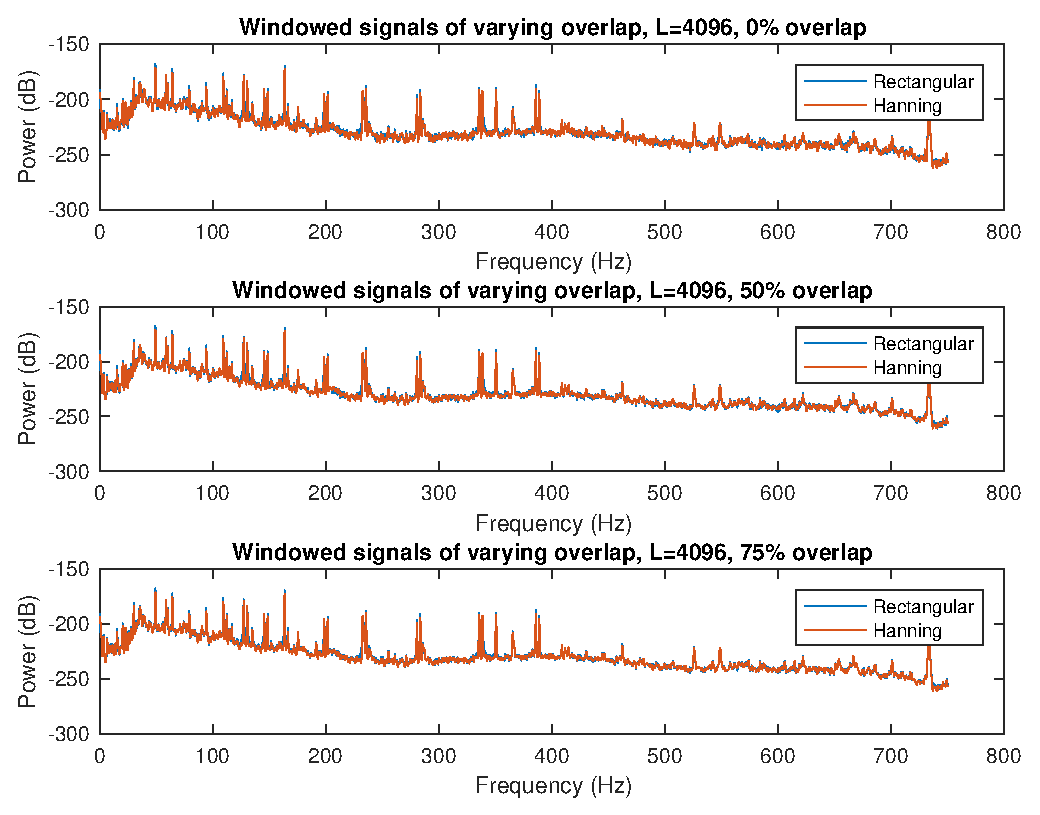
\includegraphics [width=4in]{EE125_Matlab5_05.eps}

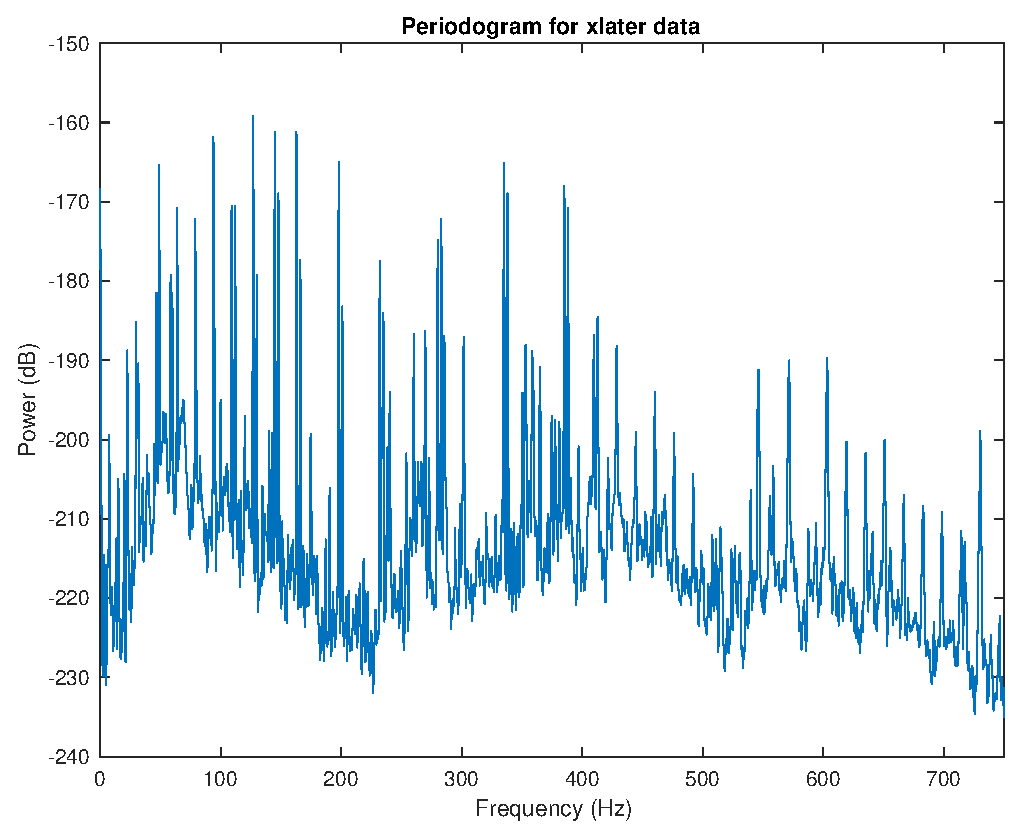
\includegraphics [width=4in]{EE125_Matlab5_06.eps}


\subsection*{Part 3: Spectrogram}

\begin{verbatim}
a = -150;
b = -75;

figure(7)
spectrogram(x,hann(L),0.75*L,L,Fs);
caxis([a b]); colorbar
title('Spectrogram for start data, hann, 75% overlap, L=4096')

figure(8)
spectrogram(xlater,hann(L),0.75*L,L,Fs);
title('Spectrogram for later data, hann, 75% overlap, L=4096')
caxis([a b]); colorbar

% The later data has a lot of consistency in the time domain and contains a
% lot more stronger components at regular intervals and higher frequencies.

load('Event59Data_20min.mat')
figure(9)
spectrogram(xbig,hann(L),0.75*L,L,Fs);
caxis([a b]); colorbar
title('Spectrogram for long data, hann, 75% overlap, L=4096')

% This spectrogram over a long period of data is really interesting because
% you can see where different events happen. Like some sort of event
% happens at around 10 minutes that causes a spike in a contained range of
% low frequency signals.
\end{verbatim}

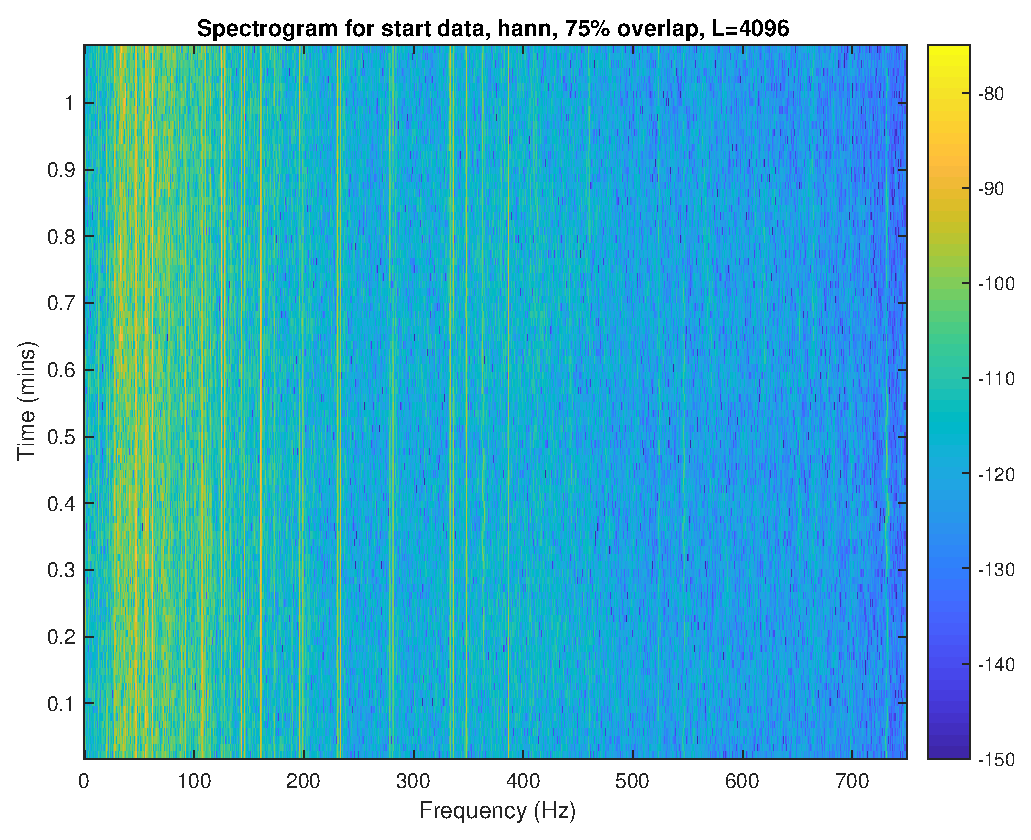
\includegraphics [width=4in]{EE125_Matlab5_07.eps}

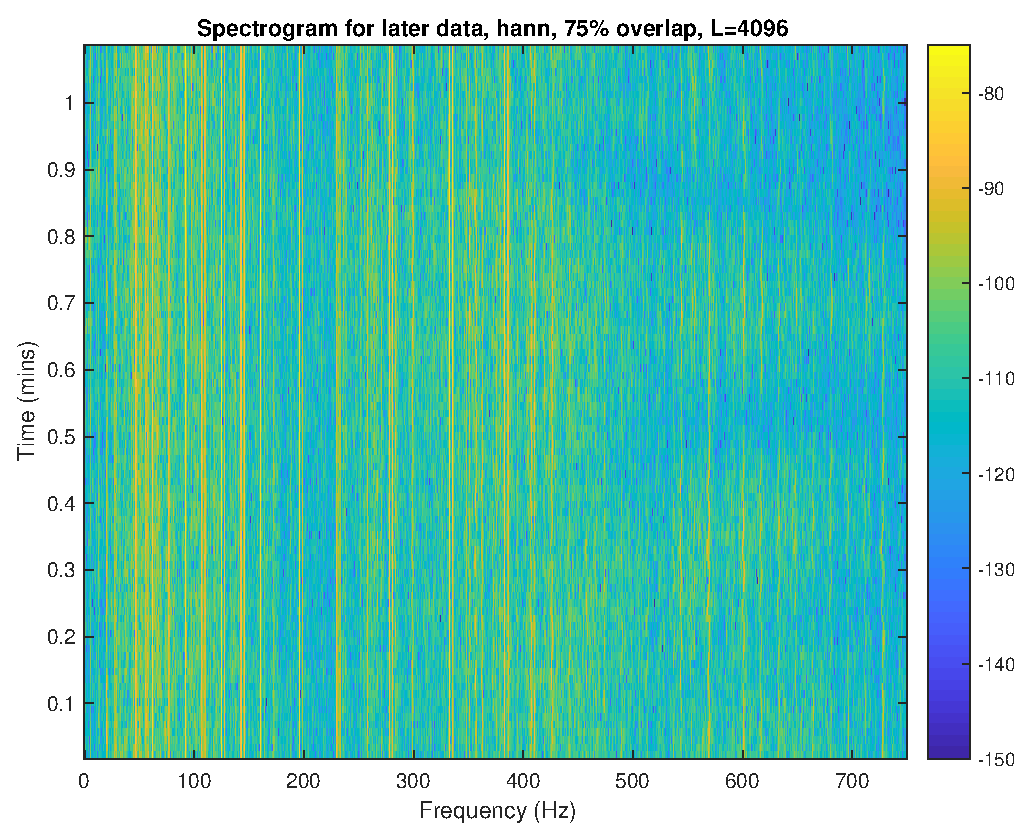
\includegraphics [width=4in]{EE125_Matlab5_08.eps}

\includegraphics [width=4in]{EE125_Matlab5_09.eps}



\end{document}
    
